% ------------------------------------------------------------------
% CAPSTONE SOFTWARE REQUIREMENTS SPECIFICATION (SRS)

% 
% This template is inspired by IEEE 29148 but simplified for use in 
% a senior software engineering capstone project. 
% 
% The goal is not to maximize document length. 
% The goal is to produce a clear, testable, and traceable set of 
% requirements that can guide design, implementation, and testing. 
% 
% Recommended workflow: 
% Stakeholder Requirements 
% -> 
% Use Cases 
% -> 
% Functional Requirements 
% -> 
% Acceptance Tests (will be in your VnV plan)
% -> 
% Traceability Matrix (will excluded traceability for tests, that will be in the VnV plan)
% 
% Students should update this document throughout the project. 
% ------------------------------------------------------------------

\documentclass[12pt]{article}

\usepackage{amsmath, mathtools}
\usepackage{amsfonts}
\usepackage{amssymb}
\usepackage{graphicx}
\usepackage{colortbl}
\usepackage{xr}
\usepackage{hyperref}
\usepackage{longtable}
\usepackage{xfrac}
\usepackage{tabularx}
\usepackage{float}
\usepackage{siunitx}
\usepackage{booktabs}
\usepackage{caption}
\usepackage{pdflscape}
\usepackage{afterpage}

\usepackage[round]{natbib}

%\usepackage{refcheck}

\hypersetup{
    bookmarks=true,         % show bookmarks bar?
      colorlinks=true,       % false: boxed links; true: colored links
    linkcolor=red,          % color of internal links (change box color with linkbordercolor)
    citecolor=green,        % color of links to bibliography
    filecolor=magenta,      % color of file links
    urlcolor=cyan           % color of external links
}

\input{../Comments.text}
\input{../Common.text}

% Used so that cross-references have a meaningful prefix

\newcounter{srnum} %Stakeholder Requirement (SR) Number
\newcommand{\srthesrnum}{SR\thesrnum}
\newcommand{\srref}[1]{SR\ref{#1}}

\newcounter{ucnum} %Use Case (UC) Number
\newcommand{\uctheucnum}{UC\theucnum}
\newcommand{\ucref}[1]{UC\ref{#1}}

\newcounter{reqnum} %Functional Requirement (FR) Number
\newcommand{\rthereqnum}{FR\thereqnum}
\newcommand{\rref}[1]{FR\ref{#1}}

\newcounter{nfrnum} %Non-Functional Requirement (NFR) Number
\newcommand{\rthenfrnum}{NFR\thenfrnum}
\newcommand{\nfrref}[1]{NFR\ref{#1}}

\newcounter{lcnum} %Likely Change (LC) Number
\newcommand{\lthelcnum}{LC\thelcnum}
\newcommand{\lcref}[1]{LC\ref{#1}}

\usepackage{fullpage}

\begin{document}

\title{Software Requirements Specification for \progname: subtitle describing software} 
\author{\authname}
\date{\today}
	
\maketitle

~\newpage

\pagenumbering{roman}

\tableofcontents

~\newpage

\section*{Revision History}

\begin{tabularx}{\textwidth}{p{3cm}p{2cm}X}
\toprule {\bf Date} & {\bf Version} & {\bf Notes}\\
\midrule
October 8 & 1.0 & Aidan: Added sections 1.1 to 1.5 (Purpose, Scope, Stakeholders, Definitions and Acronyms, and Characteristics of Intended Reader)\\
October 11 & 1.0 & Robert: Added major functional requirements\\
October 11 & 1.0 & Aidan: Grouped functional requirements into categories and added functional requirements derived from the stakeholder requirements\\
\bottomrule
\end{tabularx}

~\\
\plt{All capstone SRS documents should have a reflection appendix.}

\newpage

\pagenumbering{arabic}

\plt{This SRS template is based on the IEEE template, with input from co-pilot
  and S. Smith. It will get you started.  You should not modify the section
  headings, without first discussing the change with the course instructor.
  Modification means you are not following the template, which loses some of the
  advantage of a template, especially standardization.}

\plt{Feel free to change the appearance of the report by modifying the LaTeX
  commands.}

\plt{This template document assumes that a single program is being documented.
  If you are documenting a family of models, you should start with a commonality
  analysis.}

\plt{The SRS is not generally written, or read, sequentially.  The SRS is a
  reference document.  It is generally read in an ad hoc order, as the need
  arises.}

\plt{Guiding principles for the SRS document:
\begin{itemize}
\item Do not repeat the same information at the same abstraction level.  If
  information is repeated, the repetition should be at a different abstraction
  level.
\end{itemize}
}

\plt{The template description comments should be disabled before submitting this
  document for grading.}

\plt{You can borrow any wording from the text given in the template.  It is part
  of the template, and not considered an instance of academic integrity.  Of
  course, you need to cite the source of the template.}

\plt{When the documentation is done, it should be possible to trace back to the
  source of every piece of information.  Some information will come from
  external sources, like terminology.}

\plt{An SRS document should have the following qualities: unambiguous,
  consistent, complete, validatable, abstract and traceable.}

\plt{The overall goal of the SRS is that someone can learn,
  understand and verify the captured domain knowledge.  They should not have to
  trust the authors of the SRS on any statements.  They should be able to
  independently verify/derive every statement made.}

% ============================================================== 
\section{Introduction} 
% ==============================================================

\plt{Explain what system is being specified. State purpose, users, and project goals.}

\plt{Introduce the name of your software as \progname{}.  Using \progname{} as
a command lets you change the name if necessary and have the change propagate to
all documents.}

\plt{Include a reference to the template this work is based on.  \citet{ISOIECIEEE29148_2018}
justifies the SRS structure and \citet{ISOIECIEEE15288_2023} provides the
broader life-cycle context that underlines modern requirements engineering
practice.}

\subsection{Purpose}

DAIIM (Decentralized Artificial Intelligence Inference Marketplace) exists to reduce reliance on the small number of large organizations that currently provide most AI inference. It serves two groups of people.

For people who need machine learning predictions, DAIIM provides a way to obtain inferences for a task they define without trusting a single centralized provider. Each inference request is answered by multiple independent providers, and their predictions are combined into one consensus result. Because no single provider controls the outcome, the result is more reliable, harder to censor or manipulate, and not dependent on any one point of failure.

For people who build machine learning models, DAIIM provides an open marketplace where they can sell predictions from their models and earn money for accurate results. This gives independent providers a way to compete with large organizations and a reason to keep improving their models.

\subsection{Scope}

DAIIM allows task requesters to obtain reliable inferences by combining predictions from multiple independent inference providers.

The inputs to the system consist of task definitions, inference requests, and network participation.
Task definitions are specifications of a problem to be solved via machine learning, including the expected input and output types.
Inference requests ask the network to perform inference for a given task and include
input data or some specification of where to find the input data.
Network participation includes machine learning
predictions for individual inference requests that are supplied to the network by an individual.
The system outputs aggregated inference results and maintains information about the network.
The aggregated inference results include the final prediction for a given inference request, as well as information about the quality of the prediction.

The expected benefits are reduced reliance on centralized AI providers, improved reliability of inferences through redundant predictions from
independent providers, and incentives for providers to improve the quality, performance, availability, and cost-effectiveness of their models.

The following are outside the scope of DAIIM:
\begin{itemize}
    \item Inference tasks whose output is not a single numeric value, such as predicting a category label. Support for additional model types is a stretch goal.
    \item Inference on private or sensitive data within Trusted Execution Environments (TEEs). This is a stretch goal.
    \item DAIIM doesn't train models. It just uses model providers' existing models to make predictions for inference requests.
    \item Using a custom blockchain. DAIIM will use Solana, an existing public blockchain.
\end{itemize}

\subsection{Stakeholders} \label{sec_Stakeholders}

\subsubsection*{Primary Stakeholders}

Primary stakeholders interact with DAIIM directly.

\begin{itemize}
    \item \textbf{Task requesters} \newline
    Task requesters are people who are requesting inferences to be made for a given task, using their own input data.
    These people value consensus and reliability: they want a prediction that combines the results of multiple independent models, rather than relying on a single model that may be wrong, biased, or unavailable.
    For example, emergency management agencies would make requests to predict river levels or wildfire risk, where a single incorrect forecast can leave a community unprepared.
    Similarly, decentralized finance platforms could make requests to predict stock prices, where relying on a single source of predictions creates a risk of error or manipulation.
    Because input data is shared with inference providers, task requesters are expected to submit data that is not sensitive.

    \item \textbf{Inference providers} \newline
    Inference providers are people with computing resources and models, and want to monetize their regression models.
    These people usually have specialized or powerful models that can be used to make predictions for a given task.
\end{itemize}

\subsubsection*{Secondary Stakeholders}

Secondary stakeholders do not use DAIIM directly, but are affected by the inferences it produces or by how it handles data.

\begin{itemize}
    \item \textbf{Beneficiaries of machine learning inference} \newline
    Beneficiaries are people and organizations, such as laboratories, that rely on the results of machine learning inference without requesting inferences themselves.
    For example, a laboratory may make decisions based on biomarker predictions that a healthcare researcher obtained through DAIIM.
    These people benefit from inferences that are reliable and not controlled by a single provider.

    \item \textbf{Regulatory bodies} \newline
    Regulatory bodies are organizations that oversee machine learning inference and data privacy.
    They want to ensure that personal information and sensitive data handled by DAIIM, such as inference inputs and training data, is only accessible to the parties that need it, is encrypted, and is not retained longer than necessary to fulfill an inference request.
\end{itemize}

\subsection{Definitions and Acronyms}

\begin{longtable}{p{0.25\textwidth} p{0.65\textwidth}}
\toprule
Term & Definition\\
\midrule
AI & Artificial Intelligence.\\
ML & Machine Learning.\\
DAIIM & Decentralized Artificial Intelligence Inference Marketplace, the system specified in this document.\\
Task & A problem to be solved via machine learning, such as predicting a biomarker level or a stock price.\\
Task definition & A specification of a task, including the expected input and output types.\\
Inference & A prediction produced by a machine learning model for a given input.\\
Inference request & A request for the network to perform inference for a given task, including input data or a specification of where to find the input data.\\
Task requester & A person who requests inferences to be made for a given task.\\
Inference provider & A person with computing resources and models who supplies predictions for inference requests to the network.\\
Network participation & Machine learning predictions for individual inference requests supplied to the network by an inference provider.\\
Aggregated inference result & The final prediction for a given inference request produced by combining the predictions of multiple inference providers, together with information about the quality of the prediction.\\
Ground truth & The true, observed value that a prediction is attempting to estimate.\\
Linear regression & A machine learning model that predicts a numeric output as a linear combination of its input features.\\
Decentralized & Operating without a single central organization that coordinates or controls the system.\\
Blockchain & A distributed, append-only ledger of transactions that is maintained by a network of nodes rather than a central authority.\\
On-chain & Recorded on, or executed by, a blockchain.\\
Web3 & Applications built on blockchains, where users interact with the system through their own blockchain accounts and authorize actions by signing transactions.\\
Token & A digital asset on a blockchain, used by DAIIM to compensate inference providers.\\
TEE & Trusted Execution Environment. A secure area of a processor that protects the code and data loaded inside it from unauthorized access.\\
\bottomrule
\caption{Definitions and Acronyms} \label{tab:DefinitionsAndAcronyms}
\end{longtable}

\subsection{Characteristics of Intended Reader} \label{sec_IntendedReader}

The intended readers of this document are the software engineers, reviewers, and supervisors who will design, implement, verify, and maintain DAIIM.
Readers are expected to have:
\begin{itemize}
    \item An undergraduate-level background in software engineering, including requirements specification, software design, and testing, equivalent to the third year of a software engineering degree.
    \item Introductory knowledge of machine learning, including supervised learning, linear regression, model training versus inference, and basic error measures such as relative error, equivalent to an introductory undergraduate machine learning course.
    \item Introductory knowledge of blockchain and Web3 concepts, including blockchain transactions, accounts and wallets, transaction signing, and tokens. Familiarity with smart contract development is helpful but not required.
    \item Familiarity with web applications that run in a modern browser.
\end{itemize}
Terms specific to the domain of DAIIM are defined in Table~\ref{tab:DefinitionsAndAcronyms}.

% ============================================================== 
\section{System Overview}

This section provides general information about the system.  It identifies the
problem, the vision, and the interfaces between the system and its environment.
This section also describes user characteristics and lists the system
constraints.

\plt{The purpose of this section is to provide general information about the
  system so that the specific requirements in the later sections will be easier to
  understand. The general system description section is designed to be
  changeable independent of changes to the functional requirements documented in
  the specific system description. The general system description provides a
  context for a family of related models.  The general description can stay the
  same, while specific details are changed between family members.}

\subsection{Problem Statement}

\plt{Current situation, problem, impact, desired improvement.  You will likely borrow some text from your problem description document.}

TODO

\subsection{Product Vision}

\plt{A clear and concise statement of the product's purpose and goals.}

\plt{The goal statements are functional and nonfunctional objectives that system
  under consideration should achieve. Goals provide criteria for sufficient
  completeness of a requirements specification and for requirements pertinence.
  Goals will be refined by requirements.  The goals are written abstractly, with
  a minimal amount of technical language.  They should be understandable by
  non-domain experts.}

\plt{You will likely borrow from your goal statements in your problem
description document.}

TODO
  
\subsection{System Context}

\plt{Include users, external systems, APIs, databases, and third-party services.}

\plt{Your system context will include a figure that shows the abstract view of
  the software.  In some cases the diagram will show other external
  entities, besides the user.  For instance, when the software product is a
  library, the user will be another software program, not an actual end user.
  If there are system constraints that the software must work with external
  libraries, these libraries can also be shown on the System Context diagram.
  They should only be named with a specific library name if this is required by
  the system constraint.}

\begin{figure}[h!]
\begin{center}
 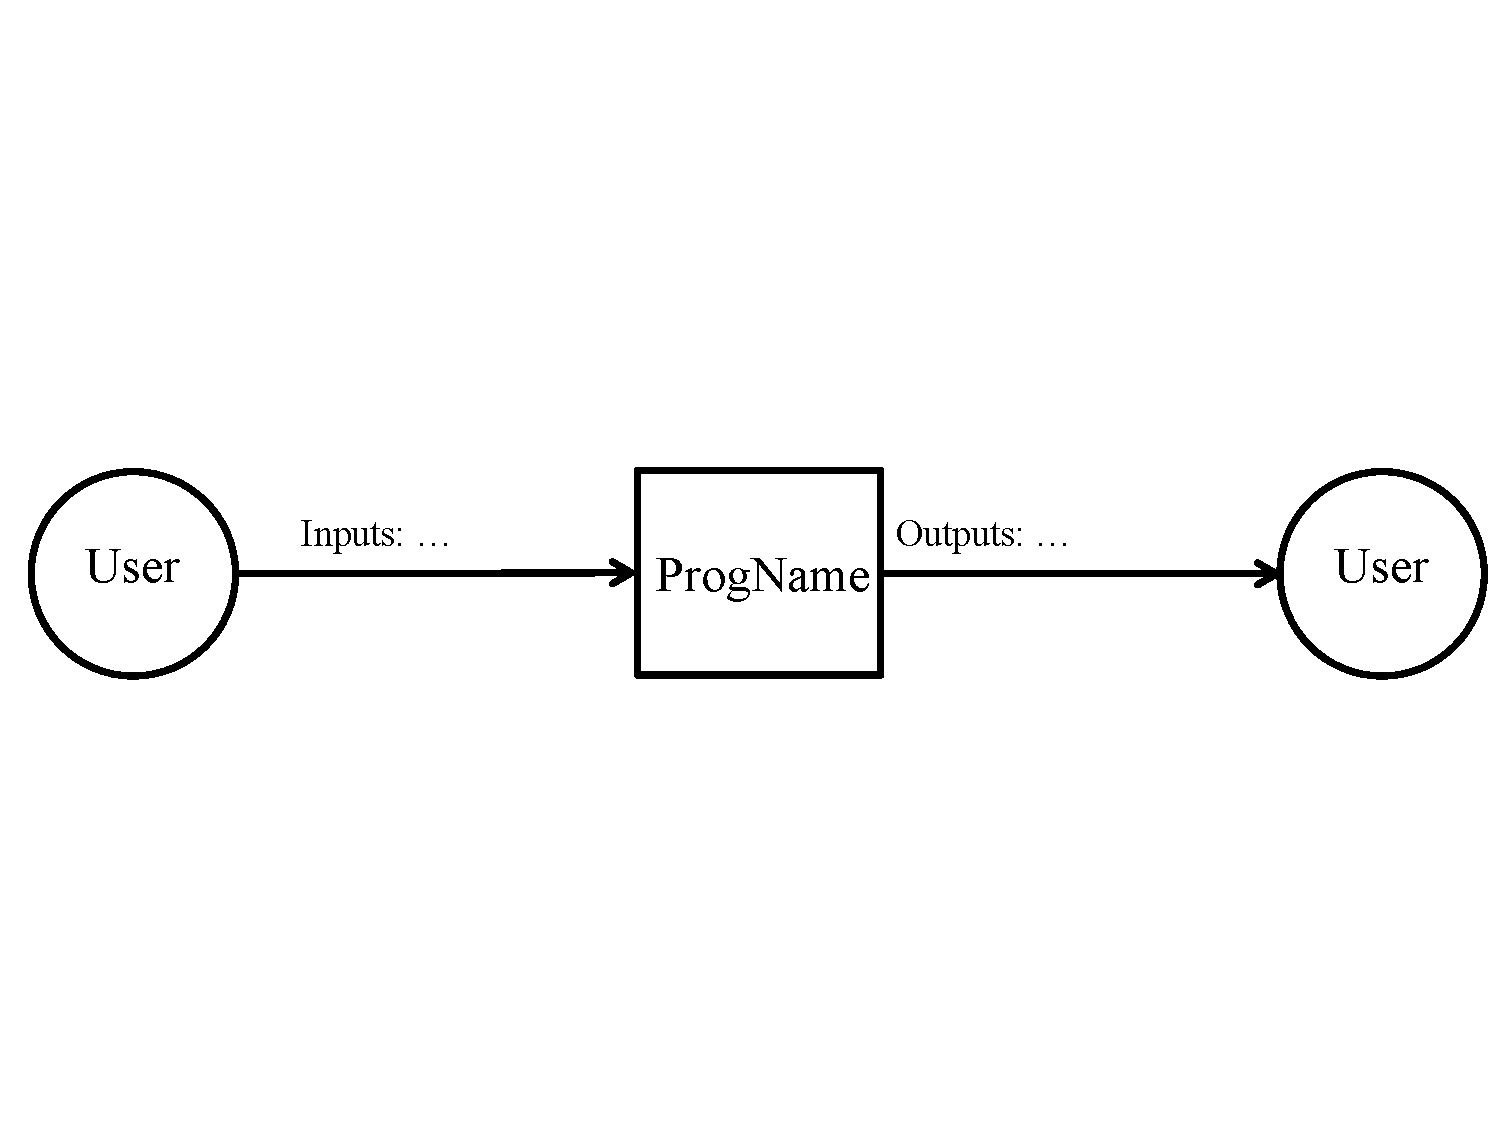
\includegraphics[width=0.6\textwidth]{SystemContextFigure}
\caption{System Context}
\label{Fig_SystemContext} 
\end{center}
\end{figure}

\plt{For each of the entities in the system context diagram its responsibilities
  should be listed.  Whenever possible the system should check for data quality,
  but for some cases the user will need to assume that responsibility.  The list
  of responsibilities should be about the inputs and outputs only, and they
  should be abstract.  Details should not be presented here.  However, the
  information should not be so abstract as to just say ``inputs'' and
  ``outputs''.  A summarizing phrase can be used to characterize the inputs.
  For instance, saying ``material properties'' provides some information, but it
  stays away from the detail of listing every required properties.}

\begin{itemize}
\item User Responsibilities:
\begin{itemize}
\item 
\end{itemize}
\item \progname{} Responsibilities:
\begin{itemize}
\item Detect data type mismatch, such as a string of characters instead of a
  floating point number
\item 
\end{itemize}
\end{itemize}

\plt{Identify in what context the software will typically be used.  Is it for
exploration? education? engineering work? scientific work?. Identify whether it
will be used for mission-critical or safety-critical applications.} 

\plt{This additional context information is needed to determine how much effort
should be devoted to the rationale section.  If the application is
safety-critical, the bar is higher.  This is currently less structured, but
analogous to, the idea to the Automotive Safety Integrity Levels (ASILs) that
McSCert uses in their automotive hazard analyses.}

\subsection{User Characteristics} \label{SecUserCharacteristics}

\plt{This section summarizes the knowledge/skills expected of the user.
  Measuring usability, which is often a required non-function requirement,
  requires knowledge of a typical user.  As mentioned above, the user is a
  different role from the ``intended reader,'' as given in
  Section~\ref{sec_IntendedReader}.  As in Section~\ref{sec_IntendedReader}, the
  user characteristics should be specific an unambiguous.  For instance, ``The
  end user of \progname{} should have an understanding of undergraduate Level 1
  Calculus and Physics.''}

\subsection{System Constraints}

\plt{System constraints differ from other type of requirements because they
  limit the developers' options in the system design and they identify how the
  eventual system must fit into the world. This is the only place in the SRS
  where design decisions can be specified.  That is, the quality requirement for
  abstraction is relaxed here.  However, system constraints should only be
  included if they are truly required.}

\plt{This is where you would mention platform constrains, and licensing
restrictions.}

% ============================================================== 
\section{Stakeholder Requirements}

This section lists the stakeholder requirements for DAIIM, grouped by the stakeholders described in Section~\ref{sec_Stakeholders}. These requirements are technology-independent and are stated from the point of view of the stakeholders.

\subsubsection*{Task Requesters}

\noindent \begin{itemize}

\item[SR\refstepcounter{srnum}\thesrnum \label{SR_DefineTask}] Task requesters shall be able to define their own machine learning task, including the type of input the task takes and the type of output it produces.

\item[SR\refstepcounter{srnum}\thesrnum \label{SR_RequestInference}] Task requesters shall be able to submit an inference request for a defined task and receive a result for that request.

\item[SR\refstepcounter{srnum}\thesrnum \label{SR_ReliableInference}] Task requesters shall receive inference results that are reliable. Each result shall be based on predictions from multiple independent inference providers, so that no single faulty or dishonest provider can determine the result.

\item[SR\refstepcounter{srnum}\thesrnum \label{SR_ResilientService}] Task requesters shall receive results for their inference requests even when some inference providers are unavailable.

\item[SR\refstepcounter{srnum}\thesrnum \label{SR_ResultQuality}] Task requesters shall receive information about the quality of each inference result, so that they can judge how much to trust it.

\item[SR\refstepcounter{srnum}\thesrnum \label{SR_NoCentralAuthority}] Task requesters shall be able to obtain inferences without relying on a single organization to coordinate the request, supply the prediction, or control the result.

\item[SR\refstepcounter{srnum}\thesrnum \label{SR_Transparency}] Task requesters shall be able to see the actions and payments they authorize, and verify that those actions and payments were carried out.

\item[SR\refstepcounter{srnum}\thesrnum \label{SR_EaseOfUse}] Task requesters shall be able to define tasks, submit inference requests, and receive results without knowledge of decentralized systems or their underlying infrastructure.

\end{itemize}

\subsubsection*{Inference Providers}

\noindent \begin{itemize}

\item[SR\refstepcounter{srnum}\thesrnum \label{SR_ProviderParticipation}] Inference providers shall be able to offer predictions from their own models for tasks defined by task requesters.

\item[SR\refstepcounter{srnum}\thesrnum \label{SR_ProviderProfit}] Inference providers shall be able to earn a profit by supplying accurate predictions to the network.

\item[SR\refstepcounter{srnum}\thesrnum \label{SR_RewardAccuracy}] Inference providers shall be rewarded according to the accuracy of their predictions, so that supplying honest, accurate predictions is more profitable than supplying dishonest or careless ones.

\item[SR\refstepcounter{srnum}\thesrnum \label{SR_AutomaticPayment}] Inference providers shall receive payment for their predictions without manual intervention from the task requester or any third party.

\end{itemize}

\subsubsection*{Secondary Stakeholders}

\noindent \begin{itemize}

\item[SR\refstepcounter{srnum}\thesrnum \label{SR_DataPrivacy}] Personal information and sensitive data handled by DAIIM, such as inference inputs and training data, shall only be accessible to the parties that need it to fulfill an inference request.

\item[SR\refstepcounter{srnum}\thesrnum \label{SR_DataProtection}] Personal information and sensitive data handled by DAIIM shall be protected from unauthorized access while it is transferred and while it is stored.

\item[SR\refstepcounter{srnum}\thesrnum \label{SR_DataRetention}] Personal information and sensitive data handled by DAIIM shall not be retained longer than necessary to fulfill the inference request it belongs to.

\end{itemize}

% ============================================================== 
\section{User Personas}

\subsection{Persona 1: Emergency Management Coordinator (Task Requester)}
\begin{itemize}
\item Name: Priya Nair
\item Description: Priya is 41 and coordinates emergency management for a mid-sized town on a flood-prone river, in a region that also has an annual wildfire season. She decides when to issue flood warnings and evacuation orders, and when to pre-position firefighting resources. She currently relies on a single forecasting service, and has to justify every decision to the town council.
\item Goals: Receive river-level forecasts 24 to 48 hours ahead, and wildfire risk estimates during fire season, that combine predictions from multiple independent sources. See how much the sources agree, so she knows how much to trust each forecast. Keep costs predictable and within the town's budget.
\item Frustrations: Her current service is a black box: it gives one number with no indication of confidence, and she has no alternative when it is wrong or unavailable. A missed flood forecast the previous spring left the town unprepared. She has no interest in learning about cryptocurrency or managing digital wallets.
\item Technical Ability: Comfortable with spreadsheets, web dashboards, and mapping tools. No programming experience and no experience with blockchain or Web3 applications.
\end{itemize}

\subsection{Persona 2: Independent Stock Forecaster (Inference Provider)}
\begin{itemize}
\item Name: Daniel Okafor
\item Description: Daniel is 29 and works as a software developer. In his spare time he builds machine learning models that predict next-day stock prices from historical market data. His models perform well in backtests, but he has no way to earn money from them other than trading with his own savings.
\item Goals: Earn a steady side income by supplying predictions from his models. Get paid automatically and promptly for good predictions. Build a visible track record that shows his models are reliable. Keep the cost of submitting each prediction low enough that participating is worthwhile.
\item Frustrations: Selling predictions usually requires connections at a fund. Trading his own money exposes him to large losses. Prediction platforms he has tried were unclear about how payouts were calculated.
\item Technical Ability: Strong Python programmer who regularly uses machine learning libraries. Owns a cryptocurrency wallet and has used decentralized finance applications.
\end{itemize}

\subsection{Persona 3: Hydrology Researcher (Inference Provider)}
\begin{itemize}
\item Name: Dr. Elena Varga
\item Description: Elena is 34 and is a postdoctoral researcher in hydrology. She specializes in forecasting streamflow in mountain rivers fed by melting snow, where standard forecasting models often perform poorly during the spring melt. Her models currently only appear in academic papers.
\item Goals: Earn supplementary income from her expertise by supplying predictions for tasks in her field, such as river-level and streamflow forecasts. Build a reputation for her models outside academia. See her research help communities prepare for floods.
\item Frustrations: Consulting contracts are slow to arrange and rarely available to early-career researchers. Her models are most valuable during unusual events, when they disagree with standard models, and she worries about being penalized for disagreeing with the majority even when she is right.
\item Technical Ability: Expert in statistical modeling, with strong Python and R skills. Has never used a cryptocurrency wallet or a blockchain application.
\end{itemize}

% ============================================================== 
\section{Use Cases}
\plt{Use cases are a way to describe the interactions between users and the system.
  They are typically written in natural language and describe the steps that a
  user takes to achieve a specific goal.  Use cases can be used to identify
  functional requirements and to create test cases.}  
\plt{Typically 8-15 substantial use cases.}

\refstepcounter{ucnum} \label{UC_Label1}
\subsection{\ucref{UC_Label1}: Example Use Case}

\textbf{Primary Actor}

TODO

\textbf{Preconditions}
\begin{itemize}
\item TODO
\end{itemize}

\textbf{Main Success Scenario}
\begin{enumerate}
\item TODO
\item TODO
\item TODO
\end{enumerate}

\textbf{Alternative Flows}
\begin{itemize}
\item TODO
\end{itemize}

\textbf{Postconditions}
\begin{itemize}
\item TODO
\end{itemize}

% ============================================================== 
\section{Functional Requirements}
\plt{Functional requirements describe what the system should do.  They are typically
expressed as a set of conditions or capabilities that the system must have.  These
requirements are usually derived from the stakeholder requirements and use cases.}

\plt{Use SHALL statements. Requirements must be atomic, testable, and traceable.}

The functional requirements are grouped by the area of DAIIM they describe.

\subsection{Accounts and Authorization}

\noindent \begin{itemize}

\item[FR\refstepcounter{reqnum}\thereqnum \label{FR_WalletAuthentication}:] The system shall allow users to authenticate by connecting their Web3 wallet and signing a verification message to prove ownership of the associated wallet address.

\item[FR\refstepcounter{reqnum}\thereqnum \label{FR_PublicAccess}:] The system shall allow unauthenticated users to browse publicly available marketplace information, including registered providers, available models, and provider reputations.

\item[FR\refstepcounter{reqnum}\thereqnum \label{FR_TransactionAuthorization}:] The system shall require authenticated users to authorize (sign) blockchain transactions through their connected wallet before executing actions that transfer tokens or modify on-chain state.

\end{itemize}

\subsection{Inference Tasks}

\noindent \begin{itemize}

\item[FR\refstepcounter{reqnum}\thereqnum \label{FR_InferenceTaskCreation}:] The system shall allow authenticated users to create new inference tasks by providing the task definition.

\item[FR\refstepcounter{reqnum}\thereqnum \label{FR_InferenceTaskDefinition}:] Each inference task definition shall specify a name, problem description, inference category or type, input schema, and output schema. Where applicable, it shall also specify the metric(s) used to evaluate predictions. The task creator may optionally provide training data, or a reference to training data, for providers to use when training or adapting models for the task.

\item[FR\refstepcounter{reqnum}\thereqnum \label{FR_TaskMinimumProviders}:] Each inference task definition shall specify the minimum number of participating providers required to fulfill an inference request for the task.

\item[FR\refstepcounter{reqnum}\thereqnum \label{FR_MinimumProvidersFloor}:] The system shall reject inference task definitions that specify a minimum number of participating providers less than 2.

\item[FR\refstepcounter{reqnum}\thereqnum \label{FR_TaskReputationTolerance}:] Each inference task definition shall specify a reputation tolerance $T$, in the units of the task's output, used to determine when a provider's reputation decreases.

\item[FR\refstepcounter{reqnum}\thereqnum \label{FR_TaskAcceptancePeriod}:] Each inference task definition shall specify the length of the acceptance period for the task's inference requests. The acceptance period for each request shall end this length of time after the request is broadcast.

\item[FR\refstepcounter{reqnum}\thereqnum \label{FR_TaskMaxPredictionTime}:] Each inference task definition shall specify the maximum prediction time for the task's inference requests, measured from the end of the acceptance period.

\item[FR\refstepcounter{reqnum}\thereqnum \label{FR_TaskBrowsing}:] The system shall allow all users to browse existing inference tasks and view each task's definition, required minimum provider stake, and number of registered providers.

\end{itemize}

\subsection{Provider Registration and Staking}

\noindent \begin{itemize}

\item[FR\refstepcounter{reqnum}\thereqnum \label{FR_InferenceTaskRegistration}:] The system shall allow authenticated users to register as inference providers for an inference task by staking the required minimum amount of tokens (reference the min \# tokens).

\item[FR\refstepcounter{reqnum}\thereqnum \label{FR_InferenceTaskRegistrationStaking}:] When a provider registers for an inference task, the system shall lock the required minimum stake for that task in escrow. The system shall return the provider's stake when the applicable conditions for releasing it are met.

\item[FR\refstepcounter{reqnum}\thereqnum \label{FR_ProviderWillingUnregistration}:] The system shall allow registered inference providers to unregister from an inference task, provided they have not accepted any acitve inference requests for that task. Upon unregistration, the provider shall be removed from the list of registered providers for the task, and their remaining staked tokens shall be returned to their token account. Upon re-registering for an inference task, the provider shall start with the baseline reputation score for that task, regardless of their previous reputation score.

\item[FR\refstepcounter{reqnum}\thereqnum \label{FR_ProviderDashboard}:] The system shall allow inference providers to view their reputation score, staked tokens, and rewards earned for each inference task they are registered for.

\end{itemize}

\subsection{Inference Requests}

\noindent \begin{itemize}

\item[FR\refstepcounter{reqnum}\thereqnum \label{FR_RequestSubmission}:] The system shall allow authenticated users to submit inference requests for an existing inference task. Each request shall include input data that conforms to the task's input schema.

\item[FR\refstepcounter{reqnum}\thereqnum \label{FR_RequestValidation}:] The system shall reject inference requests whose input data does not conform to the task's input schema.

\item[FR\refstepcounter{reqnum}\thereqnum \label{FR_RequestPayment}:] When submitting an inference request, the system shall require the requester to choose a payment amount in tokens greater than the minimum and prompt them to authorize, through their connected wallet, a transaction transferring that amount of tokens into escrow.

\item[FR\refstepcounter{reqnum}\thereqnum \label{FR_RequestBroadcast}:] After an inference request is submitted, the system shall broadcast its task definition, proposed payment amount, acceptance-period expiry time, and maximum prediction time to all providers registered for the task.

\end{itemize}

\subsection{Provider Acceptance and Predictions}

\noindent \begin{itemize}

\item[FR\refstepcounter{reqnum}\thereqnum \label{FR_AcceptancePeriodStart}:] Upon broadcast of an inference request, the system shall automatically begin the acceptance period, during which providers registered for the task may accept or decline participation.

\item[FR\refstepcounter{reqnum}\thereqnum \label{FR_AcceptancePeriodEnd}:] At the specified expiry time, the system shall end the acceptance period. All registered providers that have not accepted the request will be treated as non-participating. Inference request acceptances from inference providers outside of the acceptance period will not be considered.

\item[FR\refstepcounter{reqnum}\thereqnum \label{FR_MinimumAcceptance}:] If fewer than the task's minimum number of participating providers have accepted an inference request when the acceptance period ends, the system shall cancel the request and return the requester's escrowed payment.

\item[FR\refstepcounter{reqnum}\thereqnum \label{FR_RequestInputDistribution}:] The system shall make the request's input data, or information needed to access it, available to all providers that accepted the request during the acceptance period.

\item[FR\refstepcounter{reqnum}\thereqnum \label{FR_PredictionPhaseStart}:] Upon expiration of the acceptance period, the system shall begin collecting inferences from the set of providers that accepted the request. Predictions returned from inference providers that are not participating will be rejected.

\item[FR\refstepcounter{reqnum}\thereqnum \label{FR_PredictionSubmission}:] The system shall allow each provider that accepted an inference request to submit a prediction for that request during the prediction phase.

\item[FR\refstepcounter{reqnum}\thereqnum \label{FR_OnePredictionPerProvider}:] The system shall accept at most one prediction from each provider for a given inference request.

\item[FR\refstepcounter{reqnum}\thereqnum \label{FR_PredictionValidation}:] The system shall reject predictions that do not conform to the task's output schema.

\item[FR\refstepcounter{reqnum}\thereqnum \label{FR_PredictionPhaseEnd}:] The system shall end the prediction phase when it has received a prediction from every provider that accepted the request or when the maximum prediction time has elapsed, whichever occurs first. The system shall not accept predictions after the phase has ended.

\item[FR\refstepcounter{reqnum}\thereqnum \label{FR_MinimumPredictions}:] If fewer than the task's minimum number of participating providers have submitted predictions when the prediction phase ends, the system shall cancel the request and return the requester's escrowed payment.

\end{itemize}

\subsection{Aggregation and Results}

\noindent \begin{itemize}

\item[FR\refstepcounter{reqnum}\thereqnum \label{FR_PredictionAggregation}:] Once the prediction phase ends, the system shall aggregate the predictions into a final numerical result using a weighted aggregation algorithm in which each provider's reputation determines the weight assigned to its prediction.

\item[FR\refstepcounter{reqnum}\thereqnum \label{FR_FinalResultDelivery}:] The system shall return the final aggregated result, time elapsed since submitting the request and the number of inference providers that submitted predictions, to the user that submitted the inference request.

\item[FR\refstepcounter{reqnum}\thereqnum \label{FR_ResultSpread}:] The system shall return, with each final aggregated result, the minimum and maximum of the predictions submitted for the request.

\item[FR\refstepcounter{reqnum}\thereqnum \label{FR_RequestHistory}:] The system shall allow requesters to view the status of each inference request they have submitted and, once available, its final aggregated result.

\end{itemize}

\subsection{Reputation and Rewards}

\noindent \begin{itemize}

\item[FR\refstepcounter{reqnum}\thereqnum \label{FR_UpdateProviderReputations}:] After the final aggregated result for an inference request is computed, the system shall update the reputation score of each provider that submitted a prediction for the request. For each such provider $i$, the system shall compute $d_i$, the absolute difference between the provider's prediction and the final aggregated result, and $\bar{d}$, the average of $d_j$ over all providers that submitted predictions for the request.

\item[FR\refstepcounter{reqnum}\thereqnum \label{FR_ReputationIncrease}:] The system shall increase the reputation score of a provider whose distance $d_i$ is less than or equal to the average distance $\bar{d}$.

\item[FR\refstepcounter{reqnum}\thereqnum \label{FR_ReputationUnchanged}:] The system shall leave unchanged the reputation score of a provider whose distance $d_i$ is greater than $\bar{d}$ but less than or equal to $\bar{d} + T$, where $T$ is the task's reputation tolerance.

\item[FR\refstepcounter{reqnum}\thereqnum \label{FR_ReputationDecrease}:] The system shall decrease the reputation score of a provider whose distance $d_i$ is greater than $\bar{d} + T$, where $T$ is the task's reputation tolerance.

\item[FR\refstepcounter{reqnum}\thereqnum \label{FR_ReputationPenaltyCap}:] The system shall limit the reputation decrease a provider receives for a single inference request to at most MAX\_REPUTATION\_PENALTY, regardless of how far the provider's prediction is from the final aggregated result.

\item[FR\refstepcounter{reqnum}\thereqnum \label{FR_DistributeRewards}:] The system shall distribute the inference request's reward among all providers whose predictions contributed to the final aggregated result and whose reputation did not decrease as a result of the request, in proportion to each provider's reputation score. Each eligible provider $i$ shall receive $R \cdot r_i / \sum_j r_j$, where $R$ is the reward for the request, $r_i$ is the reputation score used to weight provider $i$'s prediction in the final aggregated result, and the sum is over all eligible providers.

\end{itemize}

\subsection{Penalties}

\noindent \begin{itemize}

\item[FR\refstepcounter{reqnum}\thereqnum \label{FR_InferenceProviderSlashing}:] The system shall slash a provider's stake only under the conditions specified in \rref{FR_SlashInvalidPrediction} and \rref{FR_SlashNoShow}, and shall burn a provider's remaining stake only under the conditions specified in \rref{FR_SlashRepeatedOffenses} and \rref{FR_ProviderForcedUnregistration}.

\item[FR\refstepcounter{reqnum}\thereqnum \label{FR_SlashInvalidPrediction}:] When the system rejects a provider's prediction under \rref{FR_PredictionValidation}, the system shall slash SLASH\_FRACTION of the provider's stake for the task and decrease the provider's reputation score.

\item[FR\refstepcounter{reqnum}\thereqnum \label{FR_SlashNoShow}:] When a provider that accepted an inference request has not submitted any prediction for the request by the end of the prediction phase, the system shall slash SLASH\_FRACTION of the provider's stake for the task and decrease the provider's reputation score.

\item[FR\refstepcounter{reqnum}\thereqnum \label{FR_SlashRepeatedOffenses}:] When a provider has been slashed for at least REPEAT\_OFFENSE\_COUNT of the last REPEAT\_OFFENSE\_WINDOW inference requests they accepted for a task, the system shall unregister the provider from the task and burn their remaining stake for the task.

\item[FR\refstepcounter{reqnum}\thereqnum \label{FR_ProviderForcedUnregistration}:] The system shall automatically unregister any inference provider whose reputation score falls below the minimum reputation threshold. Upon removal, the provider's remaining staked tokens for that inference task shall be burned.

\end{itemize}

\subsection{Transparency}

\noindent \begin{itemize}

\item[FR\refstepcounter{reqnum}\thereqnum \label{FR_TransactionPreview}:] Before prompting a user to authorize a transaction, the system shall display the action being performed and the amount of tokens being transferred.

\item[FR\refstepcounter{reqnum}\thereqnum \label{FR_TransactionStatus}:] The system shall display the status of each transaction a user has authorized until the transaction is confirmed or fails.

\item[FR\refstepcounter{reqnum}\thereqnum \label{FR_TransactionVerification}:] The system shall provide, for each transaction a user has authorized, the transaction identifier needed to look up the transaction on the blockchain.

\item[FR\refstepcounter{reqnum}\thereqnum \label{FR_OnChainRecords}:] The system shall record request payments, provider stakes, aggregated results, reputation updates, and reward distributions on the blockchain.

\end{itemize}

\subsection{Data Handling}

\noindent \begin{itemize}

\item[FR\refstepcounter{reqnum}\thereqnum \label{FR_InputAccessRestriction}:] The system shall make a request's input data available only to the requester and the providers that accepted the request.

\item[FR\refstepcounter{reqnum}\thereqnum \label{FR_InputNotOnChain}:] The system shall not store a request's input data on the blockchain in readable form.

\item[FR\refstepcounter{reqnum}\thereqnum \label{FR_InputDeletion}:] The system shall delete a request's input data from any storage the system controls once the request has been completed or cancelled.

\end{itemize}

Questions / Missing reqs: \\
- We said that the task requester gets to choose the amount of tokens they want to offer for a request - How can we express this to inference providers in a useful way? Since the total amount does not reflect how much they will earn.\\
  - Unless the requester also gets to choose exactly how many participants are necessary to complete the request.\\
- What happens if aggregation fails? Should add req for this\\
- What happens if not enough providers accept? Should add req for this\\
- Rewards distribution and provider reputation update may be changed after POC\\
- Need to define some of the thresholds used in reqs above: min reputation, amount to stake, min inference request payment etc.\\

\plt{The requirements are given labels so that they can be referenced in other
parts of the SRS.  The label names should be meaningful mnemonics, not numbers.}

% ============================================================== 
\section{Data Requirements}

\plt{The Data Requirements section describes what information the system must manage.
  It includes the major data entities, their attributes, and the relationships
  between them.  It also includes a data dictionary that defines the meaning of
  each attribute.}

\subsection{Major Data Entities}

\plt{What information must exist for the system to accomplish its goals?}

\plt{For each entity, provide a short explanation.}

\begin{itemize}
\item User
\item Song
\item Session
\item Report
\end{itemize}

\subsection{Data Dictionary}

\plt{For each entity, define all important attributes.}

\begin{longtable}{p{0.20\textwidth} p{0.20\textwidth} p{0.45\textwidth}}
\toprule
Attribute & Type & Description\\
\midrule
user\_id & UUID & Unique identifier\\
email & String & User email address\\
\bottomrule
\caption{Data Dictionary} \label{tab:DataDictionary}
\end{longtable}

\subsection{Privacy and Data Retention}

\plt{Discuss storage, retention, deletion, privacy controls,
 consent, encryption, and compliance requirements.}

TODO

% ============================================================== 
\section{Non-Functional Requirements}

\plt{You may have to add other NFRs.}

\plt{List your nonfunctional requirements.  You may consider using a fit
  criterion to make them verifiable.}

\plt{The goal is for the nonfunctional requirements to be unambiguous, abstract
  and verifiable.  This isn't easy to show succinctly, so a good strategy may be
to give a ``high level'' view of the requirement, but allow for the details to
be covered in the Verification and Validation document.}

\plt{An absolute requirement on a quality of the system is rarely needed.  For
  instance, an accuracy of 0.0101 \% is likely fine, even if the requirement is
  for 0.01 \% accuracy.  Therefore, the emphasis will often be more on
  describing now well the quality is achieved, through experimentation, and
  possibly theory, rather than meeting some bar that was defined a priori.}

\plt{You do not need an entry for correctness in your NFRs.  The purpose of the
  SRS is to record the requirements that need to be satisfied for correctness.
  Any statement of correctness would just be redundant. Rather than discuss
  correctness, you can characterize how far away from the correct (true)
  solution you are allowed to be.  This is discussed under accuracy.}

\noindent \begin{itemize}

\item[NFR\refstepcounter{nfrnum}\thenfrnum \label{NFR_Accuracy}:]
  \textbf{Accuracy} \plt{Characterize the accuracy by giving the context/use for
    the software.  Maybe something like, ``The accuracy of the computed
    solutions should meet the level needed for $<$engineering or scientific
    application$>$.  The level of accuracy achieved by \progname{} shall be
    described following the procedure given in Section~X of the Verification and
    Validation Plan.''  If you do this provide a link to the VnV plan.}

\item[NFR\refstepcounter{nfrnum}\thenfrnum \label{NFR_Usability}:] \textbf{Usability}
  Users with no knowledge of decentralized systems or their underlying
  infrastructure shall be able to define tasks, submit inference requests, and
  receive results without assistance. In usability testing with participants
  who have no prior blockchain or Web3 experience, at least
  USABILITY\_COMPLETION\_RATE of participants shall complete each of these tasks
  without assistance.

\item[NFR\refstepcounter{nfrnum}\thenfrnum \label{NFR_DataProtection}:] \textbf{Security}
  Personal information and sensitive data handled by DAIIM, such as inference
  inputs, shall be encrypted while it is transferred and while it is stored by
  the system, so that it is protected from unauthorized access.

\item[NFR\refstepcounter{nfrnum}\thenfrnum \label{NFR_Maintainability}:]
  \textbf{Maintainability} \plt{The effort required to make any of the likely
    changes listed for \progname{} should be less than FRACTION of the original
    development time.  FRACTION is then a symbolic constant that can be defined
    at the end of the report.}

\item[NFR\refstepcounter{nfrnum}\thenfrnum \label{NFR_Portability}:]
  \textbf{Portability} \plt{This NFR is easier to write than the others.  The
    systems that \progname{} should run on should be listed here.  When possible
    the specific versions of the potential operating environments should be
    given.  To make the NFR verifiable a statement could be made that the tests
    from a given section of the VnV plan can be successfully run on all of the
    possible operating environments.}

\item Other NFRs that might be discussed include verifiability,
  understandability, reusability, performance, reliability and availability, security, and accessibility.  You may have to add other NFRs.

\end{itemize}

% ============================================================== 
\section{AI and Machine Learning Requirements}

\plt{Refer to
\href{https://gitlab.cas.mcmaster.ca/courses/capstone/-/blob/main/Lectures/Lxx_DrMosserGuestLecture/2026_09_Capstone.pdf?ref_type=heads}{Dr.
Mosser's guest lecture} on AI requirements.}

\plt{Include only when applicable.}

\subsection{Model Inputs}

TODO

\subsection{Model Outputs}

TODO

\subsection{Evaluation Metrics}

\plt{Accuracy, Precision, Recall, F1, BLEU, WER, etc.}

TODO

\subsection{Known Limitations}

\plt{Explicitly document expected failure modes.}

TODO

% ============================================================== 
\section{Requirements Traceability Matrices}

\plt{The Requirements Traceability Matrix (RTM) is a table that shows the
relationship between different types of requirements. It is used to ensure that
all requirements are traceable and that no requirements are missed. The typical
flow is: Stakeholder Need -> Use Case -> Requirement}

\plt{There is also a traceability matrix between functional and nonfunctional
  requirements. The purpose of some FRs is to satisfy NFRs.  Therefore, it is
  important to show the relationship between the two.}

\plt{Further traceability to test cases and modules will be given in other
documents.}

\begin{longtable}{p{0.15\textwidth} p{0.15\textwidth} p{0.20\textwidth} p{0.20\textwidth}}

\toprule
Stakeholder Req & Use Case & Functional Req \\
\midrule
\srref{SR_Label1} & \ucref{UC_Label1} & \rref{FR_WalletAuthentication} \\
\bottomrule

\caption{Traceability Between Stakeholder Requirements, Use Cases, and
Functional Requirements} \label{tab:SR2UC2FRtm}
\end{longtable}

\begin{longtable}{p{0.20\textwidth} p{0.20\textwidth}}

\toprule
Functional Req & Nonfunctional Req \\
\midrule
\rref{FR_Label1} & \nfrref{NFR_Accuracy} \\
\bottomrule
\caption{Traceability Between Functional and Nonfunctional Requirements}
\label{tab:FR2Rtm}

\end{longtable}

% ============================================================== 

\section{Rationale}

\plt{Provide a rationale for the decisions made in the documentation.  Rationale
should be provided for scope decisions, functional requirements, nonfunctioanl
requirements, data requirements, and AI requirements.  You don't need a
rationale for everything, ust the major decisions that are not obvious.  You
should have traceability to the entities in the document that you are
referencing.}

\subsection{Provider Staking}

Inference providers must stake a minimum amount of tokens to register for an
inference task (\rref{FR_InferenceTaskRegistration}). The stake is locked in
escrow by the system's on-chain logic, rather than held by any person, and can
only be returned, slashed, or burned according to the rules in
\rref{FR_InferenceTaskRegistrationStaking},
\rref{FR_InferenceProviderSlashing},
\rref{FR_ProviderWillingUnregistration}, and
\rref{FR_ProviderForcedUnregistration}. Requiring a stake serves three
purposes:

\begin{itemize}
    \item \textbf{Resistance to fake accounts.} The final result is a
    reputation-weighted aggregate of provider predictions
    (\rref{FR_PredictionAggregation}), so anyone who controls enough providers
    for a task can control its results. Without a stake, an attacker could
    register many providers at no cost, and a provider with a low reputation
    could abandon their account and register a new one. Requiring a stake for
    every registration makes each additional provider cost real tokens, which
    makes gaining control of a task's results expensive.

    \item \textbf{Penalties for misbehaviour.} A loss of reputation alone may
    not deter a provider who has nothing else at risk. A stake allows the
    system to impose a financial penalty by slashing it
    (\rref{FR_InferenceProviderSlashing}), or burning it when a provider's
    reputation falls below the minimum threshold
    (\rref{FR_ProviderForcedUnregistration}).

    \item \textbf{Commitment to accepted requests.} If accepting an inference
    request had no cost, providers could accept every request and respond only
    when convenient, causing requests to be cancelled for having too few
    predictions (\rref{FR_MinimumPredictions}). Having a stake at risk gives
    providers a reason to submit a prediction for every request they accept.
\end{itemize}

A provider's stake does not determine the weight of their predictions;
reputation does (\rref{FR_PredictionAggregation}). This prevents providers from
gaining influence over results through wealth alone, so influence must be
earned through a history of predictions that agree with the network.

The minimum stake must balance two concerns. It must be high enough that
registering many fake providers is expensive, but low enough that honest new
providers, who have not yet earned any rewards, are not discouraged from
joining.

\subsection{Reputation Tolerance}

Each task specifies a reputation tolerance $T$ (\rref{FR_TaskReputationTolerance}),
and a provider's reputation only decreases when their distance from the final
aggregated result exceeds the average distance by more than $T$
(\rref{FR_ReputationDecrease}). Without this margin, roughly half of the
providers would lose reputation on every request, even when all predictions are
close together. $T$ is set per task because an acceptable margin depends on the
units and scale of the task's output.

\section{Likely Changes}    

\noindent \begin{itemize}

\item[LC\refstepcounter{lcnum}\thelcnum\label{LC_meaningfulLabel}:] \plt{Give
    the likely changes, with traceability to the entity that is likely to change.}

\end{itemize}

\section{Unlikely Changes}    

\noindent \begin{itemize}

\item[LC\refstepcounter{lcnum}\thelcnum\label{LC_meaningfulLabel}:] \plt{Give
    the unlikely changes.  The design can assume that the changes listed will
    not occur.}

\end{itemize}

\newpage{}

\section{Appendices}

\subsection{Appendix A: Additional Materials}

TODO

\subsection{Appendix B: Development Plan}

\plt{This section is optional.  It is used to explain the plan for developing
  the software.  In particular, this section gives a list of the order in which
  the requirements will be implemented.  In the context of a course  this is
  where you can indicate which requirements will be implemented as part of the
  course, and which will be ``faked'' as future work.  This section can be
  organized as a prioritized list of requirements, or it could show the
  requirements that will be implemented for ``phase 1'', ``phase 2'', etc.}

\subsection{Appendix C: Values of Auxiliary Constants}

\plt{Show the values of the symbolic parameters introduced in the report.}

\plt{The definition of the requirements will likely call for SYMBOLIC\_CONSTANTS.
Their values are defined in this section for easy maintenance.}

\plt{The value of FRACTION, for the Maintainability NFR would be given here.}

\begin{itemize}
\item USABILITY\_COMPLETION\_RATE: the minimum fraction of usability test participants who must complete each task without assistance (\nfrref{NFR_Usability}). To be determined.
\item MAX\_REPUTATION\_PENALTY: the maximum reputation decrease a provider can receive for a single inference request (\rref{FR_ReputationPenaltyCap}). To be determined.
\item SLASH\_FRACTION: the fraction of a provider's stake slashed for an invalid prediction or for not submitting a prediction (\rref{FR_SlashInvalidPrediction}, \rref{FR_SlashNoShow}). To be determined.
\item REPEAT\_OFFENSE\_COUNT: the number of slashing offences that causes a provider to be unregistered (\rref{FR_SlashRepeatedOffenses}). To be determined.
\item REPEAT\_OFFENSE\_WINDOW: the number of most recent accepted inference requests over which slashing offences are counted (\rref{FR_SlashRepeatedOffenses}). To be determined.
\end{itemize}

\subsection{Appendix D: Generative AI Disclosure}

\plt{Provide full transparency on how generative AI was used in the creation of
  this document.  This includes any text, figures, or tables that were generated
  by AI.  If any skills were created for AI agents to review the documentation,
  those should be disclosed here.}

\subsection{Appendix E: Reflection}

\plt{This isn't part of the SRS, but it is part of the course.}

The information in this section will be used to evaluate the team members on the
graduate attribute of Lifelong Learning.  

\input{../Reflection.text}

\input{../SRS_Reflection.text}

\newpage

\bibliographystyle {plainnat}
\bibliography {../../refs/References}

\newpage


\end{document}